%% ID: uniform_ladder
%% TITLE: A uniform ladder
%% TYPE: question
%% QUESTIONTYPE:  numerical
%% CONCEPTS: forces, friction, newtoni
%% VIDEOS: 
%% LEVEL: 4
%% TOPIC: mechanics/statics
%% ORDER: 9

\begin{problem}[A1987FMIIQ1l] %friction, ladders
{\exposition{A uniform ladder AB of mass \vari{m} rests in equilibrium. A is in contact with a smooth vertical wall and B in contact with a rough horizonal floor. The ladder lies in a vertical plane perpendicular to the wall and makes an acute angle \vari{\alpha} to the horizontal. A horizontal force \vari{P} is applied to the ladder in a direction away from and perpendicular to the wall. This force acts at the point one quarter of the way up the ladder. }

\begin{enumerate}
	\item \exposition{}
	\begin{enumerate}	
		\item \question[a]{Find, in terms of \vari{P}, \vari{m} and \vari{\alpha} the magnitudes of the normal reactions at A and B (\vari{N\s{A}} and \vari{N\s{B}} respectively) }
		\item \question[b]{Show that the frictional force on the ladder at B has magnitude $\frac{3}{4}P+\frac{1}{2}mg\cot(\alpha)$}
	\end{enumerate}
	\item \exposition{If the coefficient of friction between the ladder and the floor at B is \vari{\mu}, the value of \vari{P} is gradually increased from zero. Find how equilibrium will be broken in the following cases}
	\begin{enumerate}
		\item \question[c]{$\mu=\cot(\alpha)$}
		\item \question[d]{$\mu=4\cot(\alpha)$}
	\end{enumerate}
\end{enumerate}}
{\textit{Used with permission from UCLES, A Level Further Maths, Syllabus C, June 1987, Paper II, Question 1.}}
{\answer[a]{}
\answer[b]{}
\answer[c]{}
\answer[d]{}
\begin{figure}
	\centering
	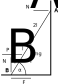
\includegraphics[width=0.3\textwidth]{Statics_ladder_slide_topple}
	\caption{}
	\label{fig:Statics_ladder_slide_topple}
\end{figure}
\begin{enumerate}
	\item
	\begin{enumerate}
		\item To start this question it is useful to define the length of the ladder as \vari{4l}. We can find the reaction force \vari{N\s{A}} at A by taking moments about point B, as in Figure \ref{fig:Statics_ladder_slide_topple}.
\begin{equation*}	
Pl\sin{\alpha} + 4N\s{A}\sin{\alpha} = 2mgl\cos{\alpha}	
\end{equation*}
\begin{equation*}	
4N\s{A}\sin{\alpha} = 2mg\cos{\alpha} - P\sin{\alpha}	
\end{equation*}
\begin{equation*}	
N\s{A} = \frac{1}{2}mg\cot{\alpha} - \frac{1}{4}P 	
\end{equation*}
We can find the reaction force \vari{N\s{B}} at B by resolving vertically on the ladder.
\begin{equation*}	
N\s{B} = mg	
\end{equation*}
		\item Resolving horizontally on the ladder:
\begin{equation*}	
N\s{A} + P = F 	
\end{equation*}
\begin{equation*}	
F = \frac{1}{2}mg\cot{\alpha} - \frac{1}{4}P + P 	
\end{equation*}
\begin{equation*}	
F = \frac{3}{4}P + \frac{1}{2}mg\cot{\alpha} 	
\end{equation*}
	\end{enumerate}
	\item Our condition for toppling is that the reaction force $N\s{A} = 0$ and moments are balanced about B.
\begin{equation*}	
Pl\sin{\alpha} = 2mgl\cos{\alpha}	
\end{equation*}
\begin{equation*}	
P = 2mg\cot{\alpha}	
\end{equation*}
Our condition for sliding is $F = F\s{max} = \mu N\s{B}$.
\begin{equation*}
\frac{3}{4}P + \frac{1}{2}mg\cot{\alpha} = \mu mg	
\end{equation*}
\begin{equation*}
 P = \frac{4}{3}mg\left(\mu - \frac{1}{2}\cot{\alpha}\right)	
 \end{equation*}
 If we equate these two values for \vari{P}, we are considering the condition where the ladder topples and slides at exactly the same moment. This will give us a critical value for \vari{\mu} for when toppling and sliding both occur.
 \begin{align*}
\frac{4}{3}\mu\s{crit} mg - \frac{2}{3}mg\cot{\alpha}&= 2mg\cot{\alpha} \\
\Rightarrow \frac{4}{3}\mu\s{crit}&= \frac{8}{3}\cot{\alpha} \\
\Rightarrow \mu\s{crit}&= 2\cot{\alpha}
 \end{align*}
 When the actual value of \vari{\mu} is greater than this critical value, the block will topple before it slides, as clearly increasing the coefficient of friction will make sliding more difficult. 
 	\begin{enumerate}
 		\item If $\mu = \cot{\alpha}$, then $\mu < \mu\s{crit}$ so equilibrium will be broken by the ladder sliding.
		\item If $\mu = 4\cot{\alpha}$, then $\mu > \mu\s{crit}$ so equilibrium will be broken by the ladder toppling.
	\end{enumerate}
\end{enumerate}
}
\end{problem}